\documentclass[11pt]{article}
\usepackage[margin=1in]{geometry}
\usepackage{amsmath,amssymb,booktabs,graphicx,setspace,caption,hyperref}
\usepackage[T1]{fontenc}
\usepackage{mathpazo}
\setlength{\parindent}{0pt}
\setlength{\parskip}{0.6em}
\captionsetup{font=small,skip=6pt}
\title{Panel MS-AR(1): common linear trend, $\rho=0.99$\\[0.4em]\large Seasonally adjusted real GDP per worker}
\author{}
\date{}
\begin{document}
\maketitle
\section{Model}
One specification. Joint panel Markov-switching AR(1) around a common linear trend. No country-specific random effects. Outcome is log seasonally adjusted real GDP per worker (2026-09-17 vintage), full sample.
\begin{align}
y_{it} &= a + g\, t + z_{it}, \\
z_{i,t+1} &= \bigl(1-\rho\bigr)\mu(s_{it}) + \rho\, z_{it} + \sigma(s_{it})\,\varepsilon_{it}, \\
s_{i,t+1} &\sim \Pi(\,\cdot\mid s_{it}).
\end{align}
Three regimes. $\rho=0.99$ is fixed and common to every regime. Median $\mu$ pinned at 0. $\sigma$ switches. Standard errors are delta-method from a numerical Hessian (not reported for the fixed $\rho$).
\clearpage
\section{Common intercept and linear trend, rho fixed at 0.99}
2026-09-17 SA panel, full sample, $y_{it}=a+gt+z_{it}$, $\rho=0.99$ fixed. 74 countries, 8670 observations, 1950-Q1--2026-Q2. Fitted countries: 74. Observations: 8670. Log-likelihood: 22607.21. Ergodic mean of the cycle $E[z]=0.7046$ (0.0694).
Common intercept $a=-6.0152$ (0.0594). Common slope $g=0.0080$ (0.0005).
\begin{table}[h]
\centering
\caption{Regime AR(1), transition matrix, and ergodic $\pi$. Columns are regimes.}
\begin{tabular}{lccc}
\toprule
 & (0) & (1) & (2) \\
\midrule
$\mu$ & -0.2514 & 0.0000 & 1.7443 \\
 & (0.0953) & --- & (0.0463) \\ \addlinespace
$\sigma$ & 0.0699 & 0.0161 & 0.0090 \\
 & (0.0020) & (0.0004) & (0.0002) \\ \addlinespace
$\rho$ (common) & 0.9900 & 0.9900 & 0.9900 \\
 &  &  &  \\ \addlinespace
$\Pi_{0\cdot}$ & 0.7351 & 0.1931 & 0.0718 \\
 & (0.0241) & (0.0222) & (0.0113) \\ \addlinespace
$\Pi_{1\cdot}$ & 0.0650 & 0.9300 & 0.0050 \\
 & (0.0066) & (0.0067) & (0.0022) \\ \addlinespace
$\Pi_{2\cdot}$ & 0.0280 & 0.0023 & 0.9698 \\
 & (0.0034) & (0.0015) & (0.0033) \\ \addlinespace
$\pi$ & 0.1492 & 0.4253 & 0.4255 \\
 & (0.0119) & (0.0305) & (0.0323) \\ \addlinespace
\bottomrule
\end{tabular}
\end{table}
\begin{figure}[h]
\centering
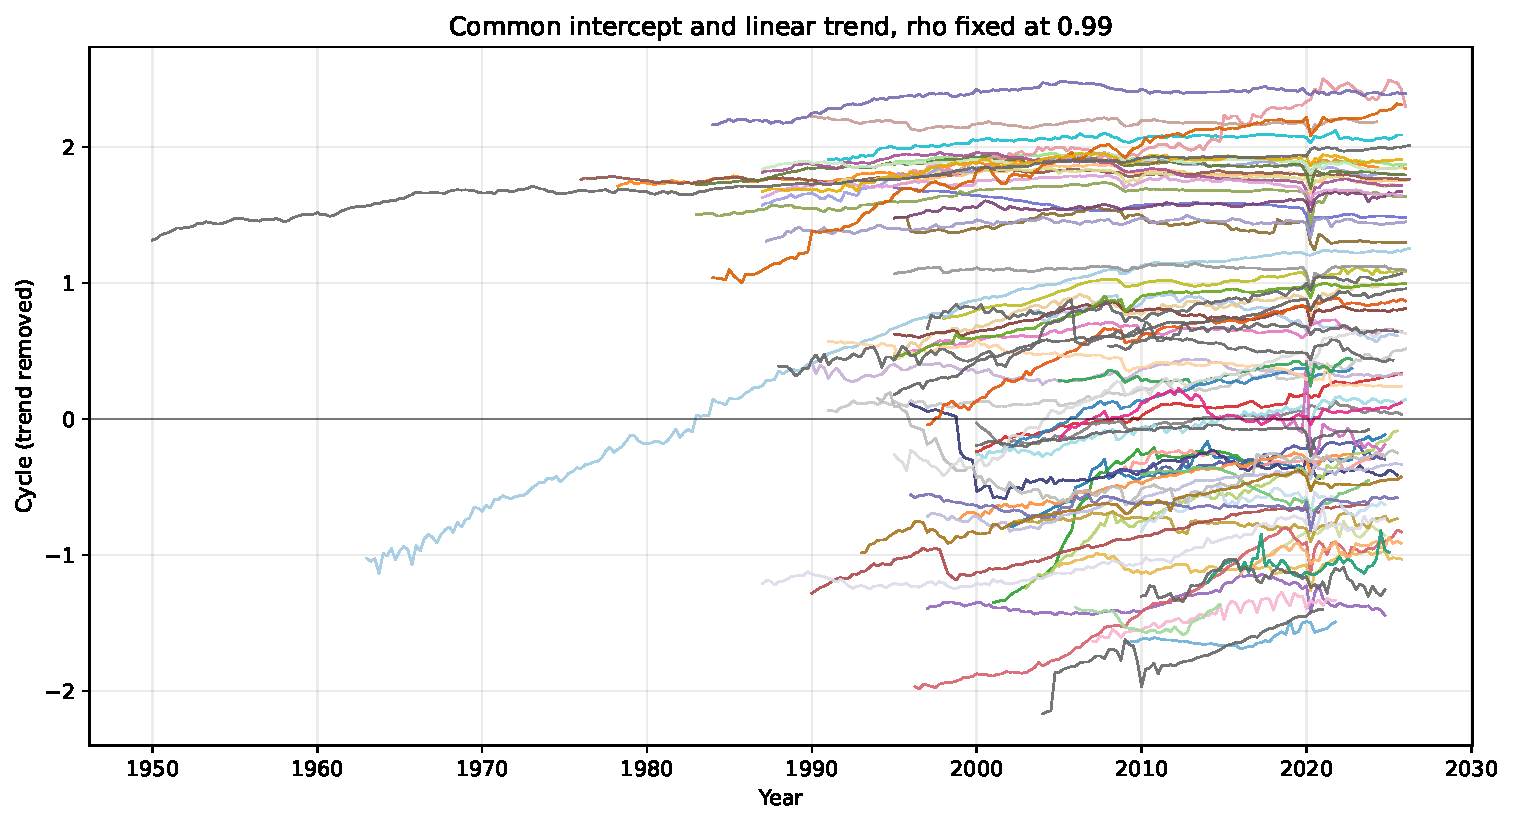
\includegraphics[width=0.75\textwidth]{figs/cycle_spec1_rho99.pdf}
\caption{Country cycles after removing the common intercept and linear trend.}
\end{figure}
\end{document}
